\subsection*{Движение по окружности и спирали}
\addcontentsline{toc}{subsection}{Движение по окружности и спирали}

\textbf{Задание:}\\
Реализовать в среде AnyLogic движение по спирали Архимеда и прямоугольной спирали.\\

\textbf{Решение:}\\
Для решения данной задачи будет рассмотрено движение по полярным координатам. Будем на каждом шаге изменять координаты $x$, $y$ и $i$.\\

Для визуализации зададим овал и будем изменять его координаты в соответствии с формулами. (Рисунок \ref{fig:spiral1})
\begin{figure}[h]
	\centering 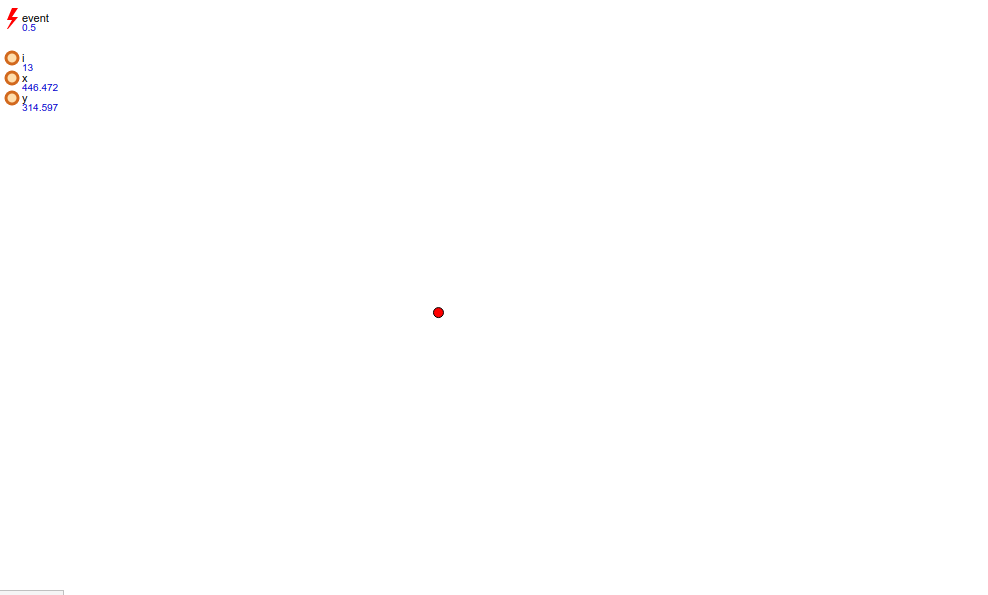
\includegraphics[scale=0.3]{spiral1}
	\caption{Схема модели в AnyLogic}
	\label{fig:spiral1}
\end{figure}

В действии события пропишем, что на каждом шаге у нас изменяется угол. В соответствии с этим мы изменяем приращение по оси $x$ и по оси $y$. Далее добавляем получившиеся приращения к текущим координатам и обновляем координаты овала. (Рисунок \ref{fig:spiral2})
\begin{figure}[h]
	\centering 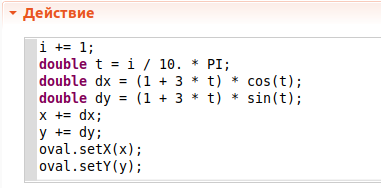
\includegraphics[scale=0.4]{spiral2}
	\caption{Алгоритм события движения по спирали Архимеда}
	\label{fig:spiral2}
\end{figure}

\newpage

Алгоритм же для движения по прямоугольной спирали заключается в том, что угол отклонения должен быть кратен 90 градусам. (Рисунок \ref{fig:spiral3})
\begin{figure}[h]
	\centering 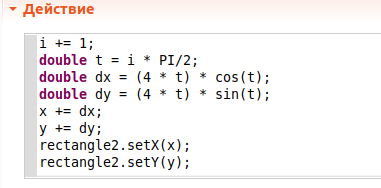
\includegraphics[scale=0.4]{spiral3}
	\caption{Алгоритм события движения по прямоугольной спирали}
	\label{fig:spiral3}
\end{figure}

Подводя итог, нам удалось воспроизвести необходимые типы движения и познакомиться с приёмами работы с элементами презентации.